\documentclass[aspectratio=169]{beamer}
\usetheme{Singapore}

\usepackage{cmap}
\usepackage[french]{babel}
\usepackage[T1]{fontenc}
\usepackage[utf8]{inputenc}
\usepackage[kerning=true]{microtype}
\usepackage{lmodern}

\usepackage{amsmath}
\usepackage{amsfonts}
\usepackage{amssymb}
\usepackage{amsthm}

\usepackage{mathtools}
\usepackage{wrapfig}
\usepackage{enumitem}

\uselanguage{French}
\languagepath{French}

%\usepackage{graphicx}

%\graphicspath{{./../report/images/}}

\AtBeginSection[]
{
  \begin{frame}
    \frametitle{Plan}
    \tableofcontents[currentsection]
  \end{frame}
}

\theoremstyle{plain}
%\newtheorem*{theorem}{Theorem}
%\newtheorem*{example}{Example}
\newtheorem*{remark}{Remarque}
\theoremstyle{definition}
%\newtheorem*{definition}{Definition}
\newtheorem*{thesis}{Thesis}

\title{\textbf{Calcul et informatique quantique:\\une introduction formelle}}
\author{Antoine Groudiev}
\institute{ENS Ulm}
\date{Janvier 2024}

\begin{document}
\frame{\titlepage}

\begin{frame}
    \frametitle{Plan}
    \tableofcontents
\end{frame}

\section{Introduction à l'informatique quantique}
\begin{frame}
    \frametitle{Introduction}
\end{frame}

\subsection{Notation de Dirac}
\begin{frame}
    \frametitle{Notation de Dirac}
\end{frame}

\subsection{Représentation vectorielle}
\begin{frame}
    \frametitle{Représentation vectorielle}
\end{frame}

\subsection{Sphère de Bloch}
\begin{frame}
    \frametitle{Visualisation avec la sphère de Bloch}
\end{frame}

\section{Modèles de calculabilité quantique}
\subsection{Circuits quantiques}
\begin{frame}
    \frametitle{Circuits quantiques}
    \begin{figure}[!ht]
        \centering
        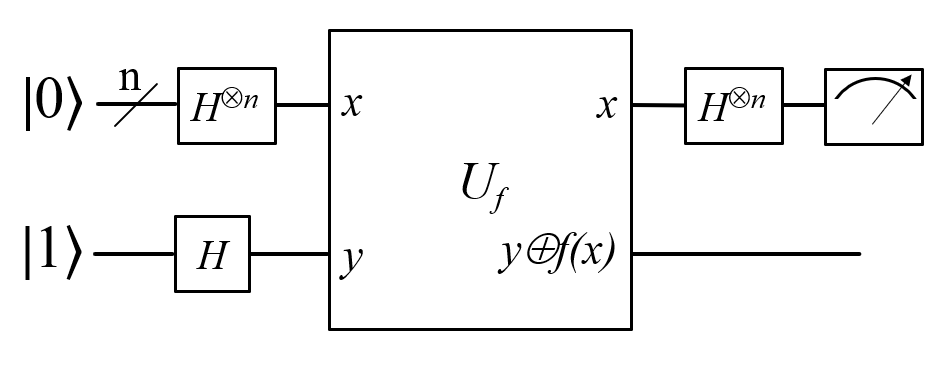
\includegraphics[scale=0.4]{deutsch-circuit-n.png}
        \caption{Un exemple de circuit (Algorithme de Deutsch-Jozsa)}
    \end{figure}
\end{frame}

\begin{frame}
    \frametitle{Porte $X$}
\end{frame}

\begin{frame}
    \frametitle{Porte $Z$}
\end{frame}

\begin{frame}
    \frametitle{Porte de Hadamard}
\end{frame}

\begin{frame}
    \frametitle{Intrication quantique}
\end{frame}

\begin{frame}
    \frametitle{Porte $CNOT$}
\end{frame}

\subsection{Langages, automates, grammaires quantiques}
\begin{frame}
    \frametitle{Langage quantique}
    \framesubtitle{Retour sur les langages classiques}
    Soit $\Sigma$ un alphabet, et $L\subseteq \Sigma^\star$ un langage. $L$ peut être défini alternativement comme un sous-ensemble de $\Sigma^\star$, ou par sa fonction caractéristique $\chi_L$:
    \begin{equation*}
        \chi_L(w) = \begin{cases*}
            1 & si $w\in L$\\
            0 & sinon
        \end{cases*}
    \end{equation*}
\end{frame}

\begin{frame}
    \frametitle{Langage quantique}
    \framesubtitle{Définition}
    On peut par analogie définir un \emph{langage quantique} comme une fonction associant des probabilités à des mots:
    \begin{definition}[Langage quantique]
        Un \emph{langage quantique} sur l'alphabet $\Sigma$ est une fonction $f$ telle que:
        \begin{equation*}
            f : \Sigma^\star \to [0, 1]
        \end{equation*}
        
    \end{definition}

    \begin{remark}
        $f$ est un langage classique lorsque $f(\Sigma^\star) \subseteq \{0, 1\}$.
    \end{remark}
\end{frame}

\begin{frame}
    \frametitle{Automate quantique fini}
    \begin{definition}[AQF]
        Un \emph{Automate Quantique Fini} $Q=(H, s_{\textnormal{init}}, H_{\textnormal{accept}}, P_{\textnormal{accept}}, \Sigma, \delta)$ constiste en:
        \begin{enumerate}[label=--, noitemsep]
            \item un espace de Hilbert $H$ de dimension $n$
            \item un vecteur initial normalisé $s_{\textnormal{init}}\in H$ (i.e. $\|s_{\textnormal{init}}\|^2=1$)
            \item un sous-espace $H_{\textnormal{accept}} \subseteq H$, et un opérateur $P_{\textnormal{accept}}$ projettant sur $H_{\textnormal{accept}}$
            \item un alphabet $\Sigma$
            \item une fonction $\delta : \Sigma \to U_n(\mathbb{C})$, associant à chaque lettre une matrice unitaire $U_a$ (c'est-à-dire $U_aU_a^\dagger = I_n$)
        \end{enumerate}
        
        On note $\delta^\star(w=w_1\cdots w_{|w|}) = \delta(w_{|w|})\cdots \delta(w_1) = U_{w_{|w|}}\cdots U_{w_1}$. Enfin, le langage reconnu par $Q$ est:
        \begin{equation*}
            f_Q : w \mapsto \|P_{\textnormal{accept}}\delta^\star(w)s_{\textnormal{init}}\|^2
        \end{equation*}
    \end{definition}
\end{frame}

\begin{frame}
    \frametitle{Langage quantique régulier et propriétés}
    \begin{definition}[LQR]
        Un \emph{Langage Quantique Régulier} est un langage quantique reconnu par un automate quantique fini
    \end{definition}

    \begin{theorem}[Clôture des LQR par produit]
        Soient $f, g$ des LQRs. Alors, le produit $fg$ est un LQR.
    \end{theorem}

    \begin{theorem}[Clôture des LQR par combinaison linéaire]
        Soient $f_i$ des LQRs, et $c_i$ des constantes telles que $\sum_i c_i \leq 1$. Alors, $\sum_i c_if_i$ est un LQR.
    \end{theorem}
\end{frame}

\begin{frame}
    \frametitle{Langage quantique régulier et propriétés}
    \begin{theorem}[Lemme de pompage quantique]
        Si $f$ est un LQR, alors pour tout mot $w\in\Sigma^\star$ et tout $\varepsilon > 0$, il existe $k\in \mathbb{N}^\star$ tel que $\|f(uw^kv) - f(uv)\| < \varepsilon$ pour tout mots $u, v$. De plus, si l'automate de $f$ est de dimension $n$, alors il existe une constante $c$ (indépendante de $\varepsilon$) telle que $k < (c\varepsilon)^{-n}$.
    \end{theorem}
\end{frame}

\begin{frame}
    \frametitle{Grammaire quantique}
    \begin{definition}[Grammaire Quantique\footnote{\url{https://xkcd.com/1090/}}]
        Une \emph{Grammaire Quantique} $G=(V, T, I, P)$ de \emph{dimensionnalité} $n$ consiste en:
        \begin{itemize}[label=--, noitemsep]
            \item un alphabet $V$ de variables
            \item un alphabet $T$ de terminaux
            \item une variable initiale $I\in V$
            \item un ensemble fini de productions $P$ de la forme $\alpha\to \beta$, où $(\alpha, \beta)\in V^\star\times (T\cup V)^\star$.
        \end{itemize}
        
    \end{definition}
\end{frame}

\begin{frame}
    À chaque production de $P$ est associée un ensemble d'amplitudes complexes $\left(c_k(\alpha\to\beta)\right)_{1\leq k\leq n}$.
    
    On définit l'amplitude d'\emph{une} suite de productions:
    \begin{equation*}
        c_k(\alpha_1 \to \dots \to \alpha_m=\beta) := \prod_{i=1}^{m-1} c_k(\alpha_i\to\alpha_{i+1})
    \end{equation*}

    Et l'amplitude d'une dérivation:
    \begin{equation*}
        c_k(\alpha\Rightarrow\beta) := \sum_{\alpha=\alpha_1 \to \dots \to \alpha_m=\beta} c_k(\alpha_1 \to \dots \to \alpha_m)
    \end{equation*}

    Enfin, $G$ \emph{génère} le langage quantique $f$ définit par:
    \begin{equation*}
        f(w) = \sum_{k=1}^n \|c_k(I\Rightarrow w)\|^2
    \end{equation*}
\end{frame}

\begin{frame}
    \frametitle{Automate à pile quantique}
\end{frame}

\begin{frame}
    \frametitle{Machine de Turing quantique}
\end{frame}

\section{Théorie de la complexité quantique}
\subsection{Classe BQP}
\begin{frame}
    \frametitle{Classe BQP (Bounded-error Quantum Polynomial time)}
\end{frame}

\begin{frame}
    \frametitle{Un problème Promise-BQP-complet}
\end{frame}

\begin{frame}
    \frametitle{Positionnement par rapport aux classes de complexité classiques}
\end{frame}

\subsection{Thèse de Church-Turing}
\begin{frame}
    \frametitle{Thèse de Church-Turing}
\end{frame}

\section{Algorithme de Deutsch-Jozsa}
\begin{frame}
    \frametitle{Description du problème}
\end{frame}

\begin{frame}
    \frametitle{Solution classique}
\end{frame}

\begin{frame}
    \frametitle{Algorithme de Deutsch}
\end{frame}

\begin{frame}
    \frametitle{Cas général ($n$ quelconque)}
\end{frame}

\end{document}